\chapter{Performance prediction through simulation: the HPL case}
\label{chapter:prediction}

The work presented in this chapter has been published at a conference\cite{cornebize:cluster19} and has been submitted
for publication in a journal. The content of this chapter is therefore a near-verbatim copy of these articles. This work
also directly follows my master thesis\cite{cornebize:master_thesis} whose main contribution is summarized in
section\ref{sec:prediction:emulation} for the sake of completeness.

\section{High Performance Linpack}%
\label{sec:prediction:hpl}

    \subsection{The benchmark}%
    \label{sub:hpl:benchmark}

        \begin{figure}[ht]
            \newcommand{\mykwfn}[1]{{\textbf{\textsf{#1}}}}%
            \SetAlFnt{\textsf}%
            \SetKwSty{mykwfn}%
            \SetKw{KwStep}{step}%
            \centering
            \begin{minipage}[m]{0.5\linewidth}
                % \vspace{0.3cm} % ugly, could not align the drawing with the algorithm with minipages or tabular...
                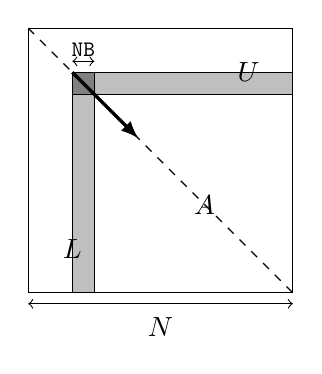
\begin{tikzpicture}[scale=0.28]
                    \draw (0, 0) -- (0, 12) -- (12, 12) -- (12, 0) -- cycle;
                    \foreach \i in {2}{
                        \draw [fill=lightgray] (\i, 0) -- (\i, 12-\i) -- (12, 12-\i) -- (12, 0) -- cycle;
                        \draw [fill=gray] (\i, 12-\i) -- (\i, 12-\i-1) -- (\i+1, 12-\i-1) -- (\i+1, 12-\i) -- cycle;
                        \draw[very thick, -latex] (\i,12-\i) -- (\i+2,12-\i-2);
                        \draw[<->] (\i, 12-\i+0.5) -- (\i+1, 12-\i+0.5) node [pos=0.5, yshift=+0.15cm] {\scalebox{.8}{\texttt{NB}}};
                    }
                    \foreach \i in {3}{
                        \draw [fill=white] (\i, 0) -- (\i, 12-\i) -- (12, 12-\i) -- (12, 0) -- cycle;
                        \draw (\i,12-\i) -- (\i,0);
                        \draw[very thick, -latex] (\i,12-\i) -- (\i+2,12-\i-2);
                    }
                    \draw[dashed] (0, 12) -- (12, 0);
                    \node(L) at (2, 2) {\ensuremath{\boldsymbol{L}}};
                    \node(U) at (10, 10) {\ensuremath{\boldsymbol{U}}};
                    \node(A) at (8, 4) {\ensuremath{\boldsymbol{A}}};
                    \draw[<->] (0, -0.5) -- (12, -0.5) node [pos=0.5, yshift=-0.3cm] {$N$};
                \end{tikzpicture}
            \end{minipage}%
            \begin{minipage}[m]{0.5\linewidth}
                \begin{algorithm}[H]
                    allocate and initialize $A$\;
                    \For{$k=N$ \KwTo $0$ \KwStep \texttt{NB}}{
                        allocate the panel\;
                        factor the panel\;
                        broadcast the panel\;
                        update the sub-matrix;
                    }
                \end{algorithm}
                \vspace{1em}
            \end{minipage}\vspace{-.5em}
            \caption{Overview of High Performance Linpack}\vspace{-1.5em}
            \label{fig:hpl_overview}
        \end{figure}

        In this work, we use the freely-available reference-implementation of HPL\cite{hpl}, which relies on MPI.  HPL
        implements a matrix factorization based on a right-looking variant of the LU factorization with row partial pivoting
        and allows multiple look-ahead depths. The principle of the factorization is depicted in
        Figure\ref{fig:hpl_overview}. It consists of a series of panel factorizations followed by an update of the trailing
        sub-matrix.  HPL uses a two-dimensional block-cyclic data distribution of $A$ and implements several custom MPI
        collective communication algorithms to efficiently overlap communications with computations.
        The main parameters of HPL are:
        \begin{itemize}
            \item \texttt{N} is the order of the square matrix $A$.
            \item \texttt{NB} is the \emph{blocking factor}, \ie the granularity at which HPL operates when panels are
                distributed or worked on.
            \item \texttt{P} and \texttt{Q} denote the number of process rows and the number of process columns,
                respectively.
            \item \texttt{RFACT} determines the panel factorization algorithm. Possible values are Crout, left- or
                right-looking.
            \item \texttt{SWAP} specifies the swapping algorithm used while pivoting. Two algorithms are available: one
                based on \emph{binary exchange} (along a virtual tree topology) and the other one based on a
                \emph{spread-and-roll} (with a higher number of parallel communications). HPL also provides a panel-size
                threshold triggering a switch from one variant to the other.
            \item \texttt{BCAST} sets the algorithm used to broadcast a panel of columns over the process columns. Legacy
                versions of the MPI standard only supported non-blocking point-to-point communications, which is why HPL
                ships with in total 6 self-implemented variants to overlap the time spent waiting for an incoming panel with
                updates to the trailing matrix: \texttt{ring}, \texttt{ring-modified}, \texttt{2-ring},
                \texttt{2-ring-modified}, \texttt{long}, and \texttt{long-modified}. The \texttt{modified} versions
                guarantee that the process right after the root (\ie the process that will become the root in the next
                iteration) receives data first and does not further participate in the broadcast. This process can thereby
                start working on the panel as soon as possible. The \texttt{ring} and \texttt{2-ring} versions each
                broadcast along the corresponding virtual topologies while the \texttt{long} version is a \emph{spread and
                roll} algorithm where messages are chopped into \texttt{Q} pieces. This generally leads to better bandwidth
                exploitation. The \texttt{ring} and \texttt{2-ring} variants rely on \texttt{MPI\_Iprobe}, meaning they
                return control if no message has been fully received yet, hence facilitating partial overlap of
                communication with computations.  In HPL 2.1 and 2.2, this capability has been deactivated for the
                \texttt{long} and \texttt{long-modified} algorithms. A comment in the source code states that some machines
                apparently get stuck when there are too many ongoing messages.
            \item \texttt{DEPTH} controls how many iterations of the outer loop can overlap with each other.
        \end{itemize}

        The sequential complexity of this factorization is \[\mathrm{flop}(N) = \frac{2}{3}N^3 + 2N^2 + \O(N)\] where $N$ is
        the order of the matrix to factorize. The time complexity can be approximated by \[T(N) \approx
        \frac{\left(\frac{2}{3}N^3 + 2N^2\right)}{P\cdot{}Q\cdot{}w} + \Theta((P+Q)\cdot{}N^2)\] where $w$ is the flop rate
        of a single node and the second term corresponds to the communication overhead which is influenced by the network
        capacity and the previously listed parameters (\texttt{RFACT}, \texttt{SWAP}, \texttt{BCAST},
        \texttt{DEPTH}, \ldots) and is very difficult to predict.

    \subsection{Typical runs on a supercomputer}%
    \label{sub:hpl:typical_runs}

        Although the TOP500 reports precise information about the core count,
        the peak performance and the effective performance, it provides almost
        no information on how (software versions, HPL parameters, etc.) this
        performance was achieved. Some colleagues agreed to provide us with
        the HPL configuration they used and the output they submitted for
        ranking (see Table\ref{fig:typical_run}).
        In June 2013, the Stampede supercomputer at TACC was ranked
        6th in the TOP500 by achieving \NSI{5168.1}{\tera\flops}. In November
        2017, the Theta supercomputer at ANL was ranked 18th with a performance of \NSI{5884.6}{\tera\flops}
        but required a 28-hour run on the
        whole machine. Finally, we ran HPL ourselves on a Grid'5000 cluster
        named Dahu whose software stack could be fully controlled.

        \begin{table}[hb]
            \caption{Typical runs of HPL}
            \label{fig:typical_run}
            \scalebox{.9}{\begin{tabular}{l|lll}
                \multicolumn{1}{l|}{} & Stampede@TACC & Theta@ANL & Dahu@G5K\\
                \hline
                \texttt{Rpeak}     & \NSI{8520.1}{\tera\flops} & \NSI{9627.2}{\tera\flops} & \NSI{62.26}{\tera\flops}              \\
                $N$         & \Num{3875000}                & \Num{8360352}                & \Num{500000}            \\
                \texttt{NB}        & \Num{1024}                    & 336                      & 128                \\
                $P\times Q$             & 77$\times$78                  & 32$\times$101                 & 32$\times$32            \\
                \texttt{RFACT}     & Crout                    & Left                     & Right              \\
                \texttt{SWAP}      & Binary-exch.             & Binary-exch.             & Binary-exch.       \\
                \texttt{BCAST}     & Long modified            & 2 Ring modified          & 2 Ring             \\
                \texttt{DEPTH}     & 0                        & 0                        & 1                  \\
                \hline
                \texttt{Rmax}      & \NSI{5168.1}{\tera\flops} & \NSI{5884.6}{\tera\flops} & \NSI{24.55}{\tera\flops}              \\
                Duration   & 2 hours                  & 28 hours                 & 1 hour             \\
                Memory    & \NSI{120}{\tera\byte}     & \NSI{559}{\tera\byte}     & \NSI{2}{\tera\byte} \\
                MPI ranks & 1/node                & 1/node                   & 1/core             \\
            \end{tabular}}
        \end{table}


        The performance typically achieved by supercomputers (\texttt{Rmax}) needs to be compared to the much larger
        peak performance (\texttt{Rpeak}). This difference can be attributed to the node usage, to the MPI library, to
        the network topology that may be unable to deal with the intense communication workload, to load imbalance among
        nodes (\eg due to a defect, system noise, \ldots), to the algorithmic structure of HPL, etc. All these factors
        make it difficult to know precisely what performance to expect without running the application at scale.  It is
        clear that due to the level of complexity of both HPL and the underlying hardware, simple performance models
        (analytic expressions based on $N, P, Q$ and estimations of platform characteristics) may be able to provide
        trends but can by no means accurately predict the performance for each configuration (\eg consider the exact
        effect of HPL's six different broadcast algorithms on network contention). Additionally, these expressions do
        not allow engineers to improve the performance through actively identifying performance bottlenecks.  For
        complex optimizations such as partially non-blocking collective communication algorithms intertwined with
        computations, a very faithful modeling of both the application and the platform is required. One goal of this
        thesis was to simulate systems at the scale of Stampede. Given the scale of this scenario (3,785~steps on
        6,006 nodes in two hours), detailed simulations quickly become intractable without significant effort.



\section{Related work}%
\label{sec:prediction:related_work}

    \subsection{Performance prediction}%
    \label{sub:performance_prediction}

        A first approach for estimating the performance of applications like HPL is statistical modeling of the
        application as a whole\cite{hpl_prediction}.  By running the application several times with small and medium
        problem sizes (of a few iterations of large problem sizes) and using simple linear regressions, it is possible
        to predict its makespan for larger sizes with an error of only a few percents and a relatively low cost.
        Unfortunately, the predictions are limited to the same application configuration and studying the influence of
        the number of rows and columns of the virtual grid or of the broadcast algorithms requires a new model and new
        (costly) runs using the whole target machine.  Furthermore, this approach does not allow to study what-if
        scenarios (\eg to evaluate what would happen if the network bandwidth was increased or if node heterogeneity was
        decreased) that are particularly useful when investigating potential performance improvements.

        Simulation provides the details and flexibility missing to such black-box modeling approach. Performance
        prediction of MPI applications through simulation has been widely studied over the last decades but two
        approaches can be distinguished in the literature: offline and online simulation.

        With the most common approach, \emph{offline simulation}, a trace of the application is first obtained on a real
        platform. This trace comprises sequences of MPI operations and CPU bursts and is given as an input to a
        simulator that implements performance models for the CPUs and the network to derive predictions. Researchers
        interested in finding out how their application reacts to changes to the underlying platform can replay the
        trace on commodity hardware at will with different platform models.
        Most HPC simulators available today, notably BigSim\cite{bigsim_04}, Dimemas\cite{dimemas} and
        CODES\cite{CODES}, rely on this approach.  The main limitation of this approach comes from the trace acquisition
        requirement. Not only is a large machine required but the compressed trace of a few iterations (out of several
        thousands) of HPL typically reaches a few hundred MB, making this approach quickly impractical\cite{suter}.
        Worse, tracing an application provides only information about its behavior at the time of the run: slight
        modifications (\eg to communication patterns) may make the trace inaccurate. The behavior of simple applications
        (\eg \texttt{stencil}) can be extrapolated from small-scale traces\cite{scalaextrap,pmac_lspp13} but this fails
        if the execution is non-deterministic, \eg whenever the application relies on non-blocking communication
        patterns, which is unfortunately the case for HPL.

        The second approach discussed in the literature is \emph{online simulation}.  Here, the application is executed
        (emulated) on top of a simulator that is responsible to determine when each process is run. This approach allows
        researchers to study directly the behavior of MPI applications but only a few recent simulators such as SST
        Macro\cite{sstmacro}, SimGrid/SMPI\cite{simgrid} and the closed-source xSim\cite{xsim} support it. To the best
        of our knowledge, only SST Macro and SimGrid/SMPI are mature enough to faithfully emulate HPL. This work relies
        on SimGrid as its performance models and its emulation capabilities seemed quite solid but the proposed
        developments would a priori also be possible with SST.  Note that the HPL emulation described in
        Section\ref{sec:prediction:emulation} should not be confused with the application
        skeletonization\cite{sst_skeleton} commonly used with SST. Skeletons are code extractions of the most important
        parts of a complex application whereas we only modify a few dozens of lines of HPL before emulating it with
        SMPI. Finally, it is important to understand that the proposed approach is intended to help studies at the level
        of the whole machine and application, not the influence of microarchitectural details as intended by
        MUSA\cite{musa_16}.

    \subsection{Simgrid/SMPI}%
    \label{sub:simgrid_smpi}

        SimGrid\cite{simgrid} is a flexible and open-source simulation framework that was originally designed in 2000 to
        study scheduling heuristics tailored to heterogeneous grid computing environments but has later been extended to
        study cloud and HPC infrastructures. The main development goal for SimGrid has been to provide validated performance
        models particularly for scenarios making heavy use of the network.  Such a validation usually consists of comparing
        simulation predictions with results from real experiments to confirm or debunk network and application models.

        SMPI, a simulator based on SimGrid, has been developed and used to simulate unmodified MPI applications written in
        C/C++ or FORTRAN\cite{smpi}.
        The complex network optimizations done in real MPI implementations need to be considered when predicting the
        performance of MPI applications.  For instance, the "eager" and "rendez-vous" protocols are selected based on the
        message size, with each protocol having its own synchronization semantics, which strongly impact performance.  SMPI
        supports different performance modes through a generalization of the LogGPS model.  Another difficult issue is to
        model network topologies and contention. SMPI relies on SimGrid's communication models where each ongoing
        communication is represented as a whole (as opposed to single packets) by a \emph{flow}. Assuming steady-state,
        contention between active communications can then be modeled as a bandwidth sharing problem that accounts for
        non-trivial phenomena (\eg cross-traffic interference\cite{Velho_TOMACS13}). If needed, communications that start or
        end trigger a re-computation of the bandwidth share.  In this fluid model, the time to simulate a message passing
        through the network is independent of its size, which is advantageous for large-scale applications frequently
        sending large messages and orders of magnitude faster than packet-level simulation.  SimGrid does not model
        transient phenomena incurred by the network protocol but accounts for network topology and heterogeneity. Special
        attention to the modeling of collective communication algorithms has also been paid in SMPI, but this is of little
        significance in this article as HPL ships with its own implementation of collective operations.

        SMPI maps every MPI rank of the application onto a lightweight simulation thread. These threads are then run one at
        a time, \ie in mutual exclusion.  Every time a thread enters an MPI call, SMPI takes control and the time that was
        spent computing (isolated from the other threads) since the previous MPI call is injected into the simulator as a
        virtual delay.  This time may be scaled up or down depending on the speed of the simulated machine with respect to
        the simulation machine.
        Recent results report consistent performance predictions within a few percent for standard benchmarks on small-scale
        clusters (up to \(12\times12\) cores \cite{heinrich:hal-01523608} and up to \(128\times1\) cores \cite{smpi}). In
        this thesis, I validate this approach at a much larger scale with HPL, whose emulation comes with at least two
        challenges:
        \begin{itemize}
        \item The time-complexity of the algorithm is \(\Theta(N^3)\) and \(\Theta(N^2)\) communications are performed, with
            \(N\) being very large. The execution on the Stampede cluster took roughly two hours on \Num{6006}~compute
            nodes. Using only a single node, a naive emulation of HPL at the scale of the Stampede run would take about
            500 days if perfect scaling was reached.
        \item The tremendous memory consumption and amount of memory accesses need to be drastically reduced.
        \end{itemize}

\section{Emulating HPL at large scale}%
\label{sec:prediction:emulation}

    some text...

\section{Modeling HPL kernels and communications}%
\label{sec:prediction:modeling}

    some text...

\section{Validation}%
\label{sec:prediction:validation}

    some text...

\section{Sensibility analysis}%
\label{sec:prediction:sensibility}

    some text...
